\section{Particle composition and detector response of hadronic recoil}

This section examines the particle composition and the detector response of the leading jet that balance the $Z$~boson in the fiducial region of the analysis.
The Powheg $Z\to \mu\mu$ sample is used. The particle origin of each track is obtained using the \texttt{truthParticleLink} to find the truth identification of each reconstructed track (see section~\ref{sec:samples}). In addition to the standard event preselection described in section~\ref{sec:selection}, extra cuts are used to make sure the leading reconstructed jet matches the leading particle jet in each event.
%To ensure the closet matching between the leading reconstructed jet and leading truth jet, and always have very good DR between them, the cut on ratio of
This is achieved by requiring $|y_\mathrm{j1}|<2.1$ and $\pTlj / \pTsj < 0.7$. The selection is applied on reconstructed level. However, due to the additional criterion, the leading particle-level (truth) jet will always match the leading reco jet. Note that the jets will have a very high \pt{} since the event selection includes the selection $\pTll > \SI{165}{\GeV}$, and the jet will have a similar \pt{} to that of the $Z$~boson. 

Further events are required to pass track-to-vertex association (TTVA) recommendations as described in section~\ref{subsubsec:trigger}. There are three recommending working points for \texttt{TTVA}, however studies have been done for two only i.e \texttt{loose} and \texttt{tight TTVA} selection.  

Particles are classified depending to their type in the following categories: \texttt{pion} for $\pi^+$ and $\pi^-$; \texttt{kaon} for charged kaons; \texttt{proton};
\texttt{mu} for $\mu^-$ or $\mu^+$; \texttt{e} for $e^-$ or $e^+$;
strange for any charge hadron with strange content other than kaons; \texttt{neutral} for any neutral hadron; \texttt{gam} for photons. As mentioned above, tracks are classified in the same categories using the \texttt{truthParticleLink}. In case there is no truth particle match, it is labelled unmatched. This includes contributions from pileup particles and fake tracks (and possibly secondaries).

All of the reconstructed tracks inside leading jet as well as charged-particles in the associated particle-level jets that are not matched to reconstructed tracks are used for the plots shown in this section. 

Figures~\ref{fig:r_pion_kaon} to ~\ref{fig:r_trackjet} are showing the detector response for each particle category for tight and loose TTVA working point. The pion and kaon response for \texttt{loose} and \texttt{tight TTVA} is ~94\% and ~93\% respectively.

Figure~\ref{fig:frac_unmatchedtracks} depicts fraction of unmatched track w.r.t reco level jet, which indicates ~3\% and ~8\% unmatched tracks for \texttt{tight} and \texttt{loose TTVA} working point respectively. Since \texttt{tight TTVA}  selection reduces ~5\% unmatched tracks as compare to \texttt{loose TTVA}, therefore for the current analysis we are using \texttt{tight TTVA} working point. 

\begin{figure}[b]
\centering
\includegraphics[scale=0.3, page=4]{figures/jet_comp_study_powheg_Tight_pTFraction_mc16e.pdf}
\includegraphics[scale=0.3, page=5]{figures/jet_comp_study_powheg_Tight_pTFraction_mc16e.pdf}
\caption {The response of pions (left) and  kaons (right) as a function of jet \pT. We can see that \texttt{tight TTVA} has $\approx 42$\% tracking efficiency while \texttt{loose TTVA} improved it by $\approx 1$\%}
\label{fig:r_pion_kaon}
\end{figure}

\begin{figure}[b]
\centering
\includegraphics[scale=0.3, page=6]{figures/jet_comp_study_powheg_Tight_pTFraction_mc16e.pdf}
\includegraphics[scale=0.3, page=7]{figures/jet_comp_study_powheg_Tight_pTFraction_mc16e.pdf}
\caption {The response of protons (left) and muons (right) as a function of jet \pT.}
\label{fig:r_proton_muon}
\end{figure}

\begin{figure}[b]
\centering
\includegraphics[scale=0.3, page=8]{figures/jet_comp_study_powheg_Tight_pTFraction_mc16e.pdf}
\includegraphics[scale=0.3, page=9]{figures/jet_comp_study_powheg_Tight_pTFraction_mc16e.pdf}
\caption {The response of electrons (left) and strange particles (right) as a function of jet \pT.}
\label{fig:r_electron_starnge}
\end{figure}

\begin{figure}[b]
\centering
\includegraphics[scale=0.3, page=16]{figures/jet_comp_study_powheg_Tight_pTFraction_mc16e.pdf}
\caption {The fraction of unmatched tracks w.r.t reco level jet as a function of jet \pT. We can see that \texttt{loose TTVA} has $\approx 8$\% unmatched tracks, while \texttt{tight TTVA} reduced unmatched tracks by $\approx 5$\%.}
\label{fig:frac_unmatchedtracks}
\end{figure}

\begin{figure}[b]
\centering
\includegraphics[scale=0.3, page=17]{figures/jet_comp_study_powheg_Tight_pTFraction_mc16e.pdf}
\caption {The response of  all the reconstructed tracks w.r.t charged particles as a function of jet \pT. The \texttt{loose TTVA} shows $\approx 4$\% higher track jet response than \texttt{tight TTVA}. However \texttt{loose TTVA} introduces $\approx 5$\% more tracking inefficiencies as compare to \texttt{tight TTVA} as shown in Figure~\ref{fig:frac_unmatchedtracks}.}
\label{fig:r_trackjet}
\end{figure}

For the following composition plots \texttt{tight TTVA} selection is used to study jet composition for different particles and the comparison of individual particles fraction is shown at \texttt{reco} and \texttt{truth} level.

Figure~\ref{fig:truthJetComp} shows the jet composition as a fraction of the particle multiplicity (left) and their momentum (right) as a function of the leading truth jet \pT{}. The $\approx 50$\% of reconstructed tracks make up pions about of the total, kaons are about $\approx 8$\% of the total and the rest $\approx 42$\% are neutral particles. The momentum fraction as a function of jet pT is shown in right in Figure~\ref{fig:truthJetComp}. The momentum fraction for different particles varies slightly as compare to multiplicity fraction.

\begin{figure}[b]
\centering
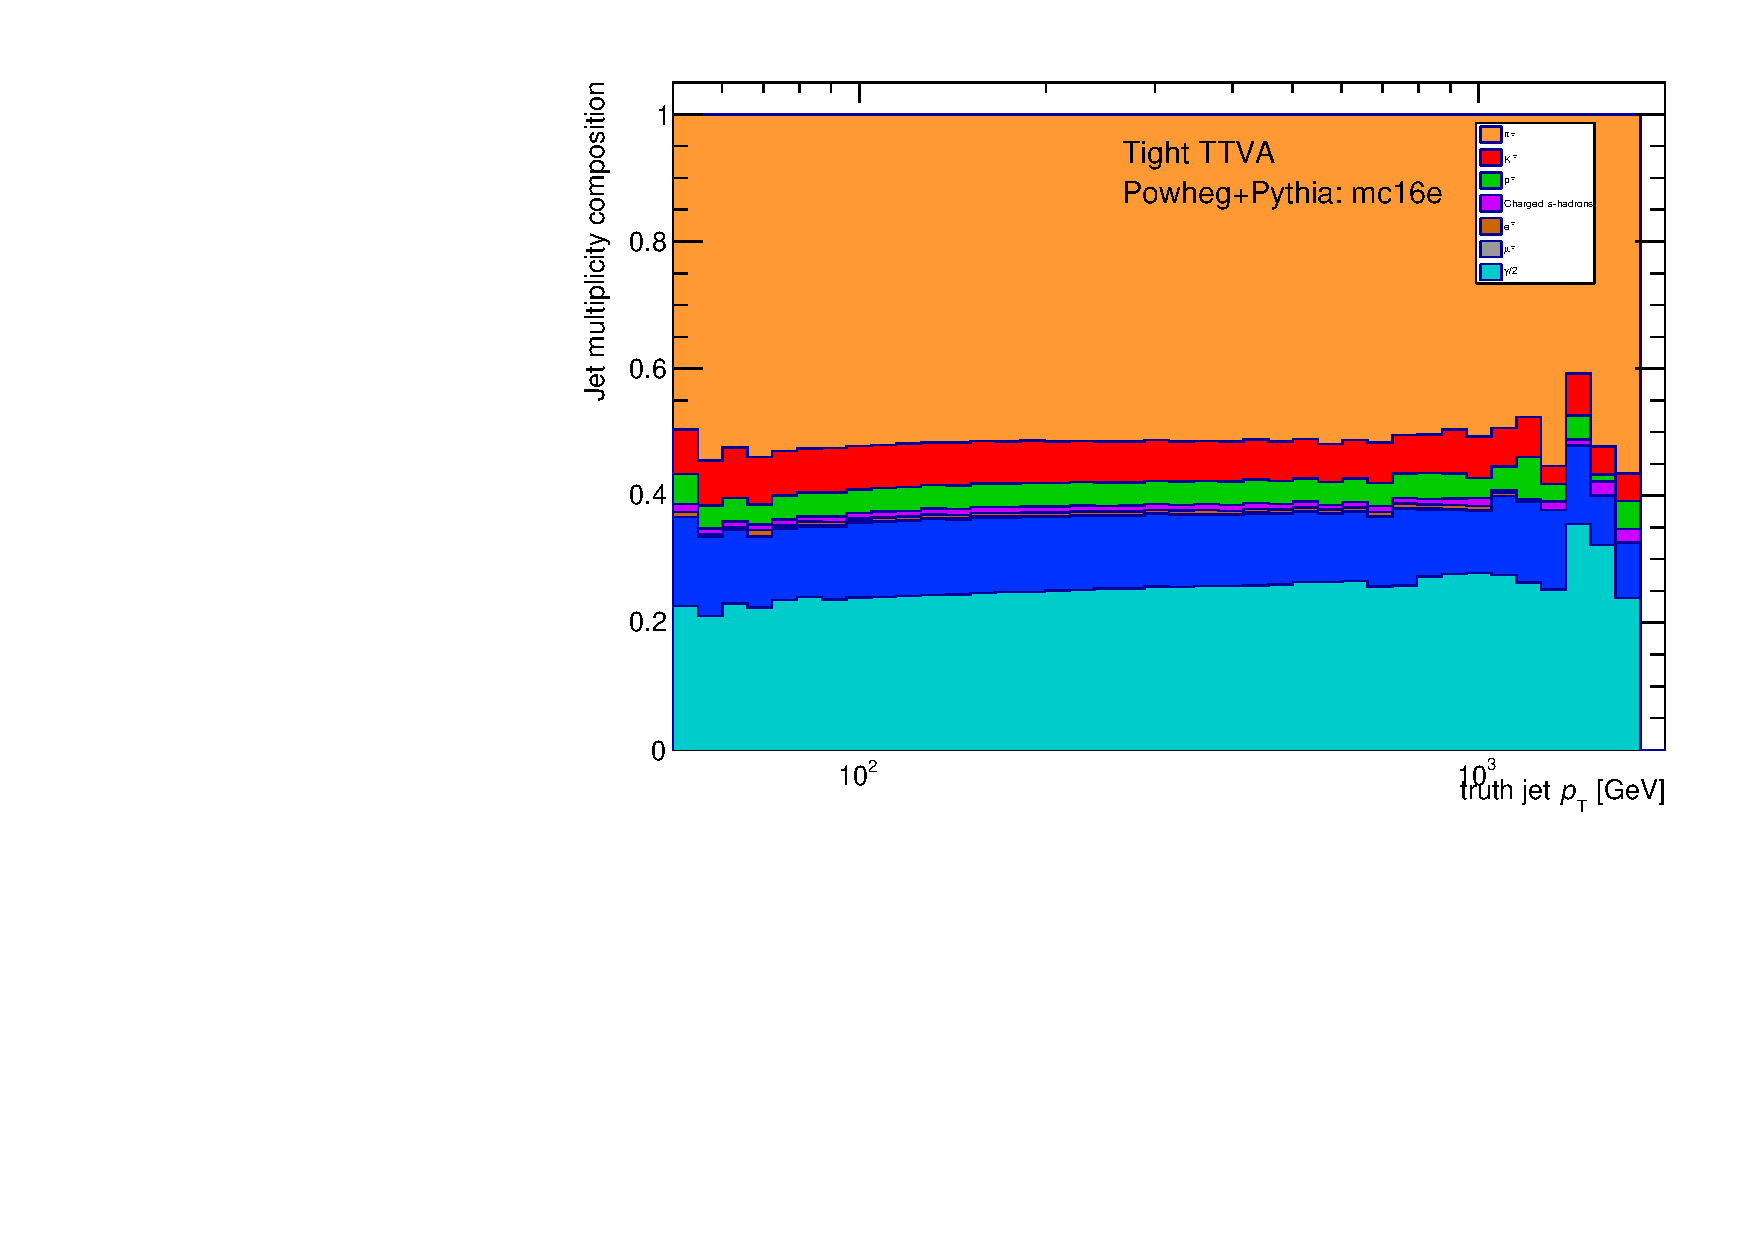
\includegraphics[width=0.48\textwidth,page=1]{figures/jet_comp_study_fixedGamma.pdf}
\includegraphics[width=0.48\textwidth,page=2]{figures/jet_comp_study_fixedGamma.pdf}%
\caption{Composition of the leading jet in terms of particle multiplicity (left) and \pt{} (right) as a function of jet \pt{}. The photon multiplicity is divided by 2 in the left plot, since most photons are produced in pairs by a neutral hadron (e.g.\ $\pi\to\gamma\gamma$).
We can see that $\approx 42$\% of the jet \pt{} is carried by neutral particles.}
\label{fig:truthJetComp}
\end{figure}

Figure~\ref{fig:chargedparticles} shows the fraction of the particle multiplicity (left) and their \pT{} as a function of the truth jet \pT in the particle-level jet. 

\begin{figure}[b]
\centering
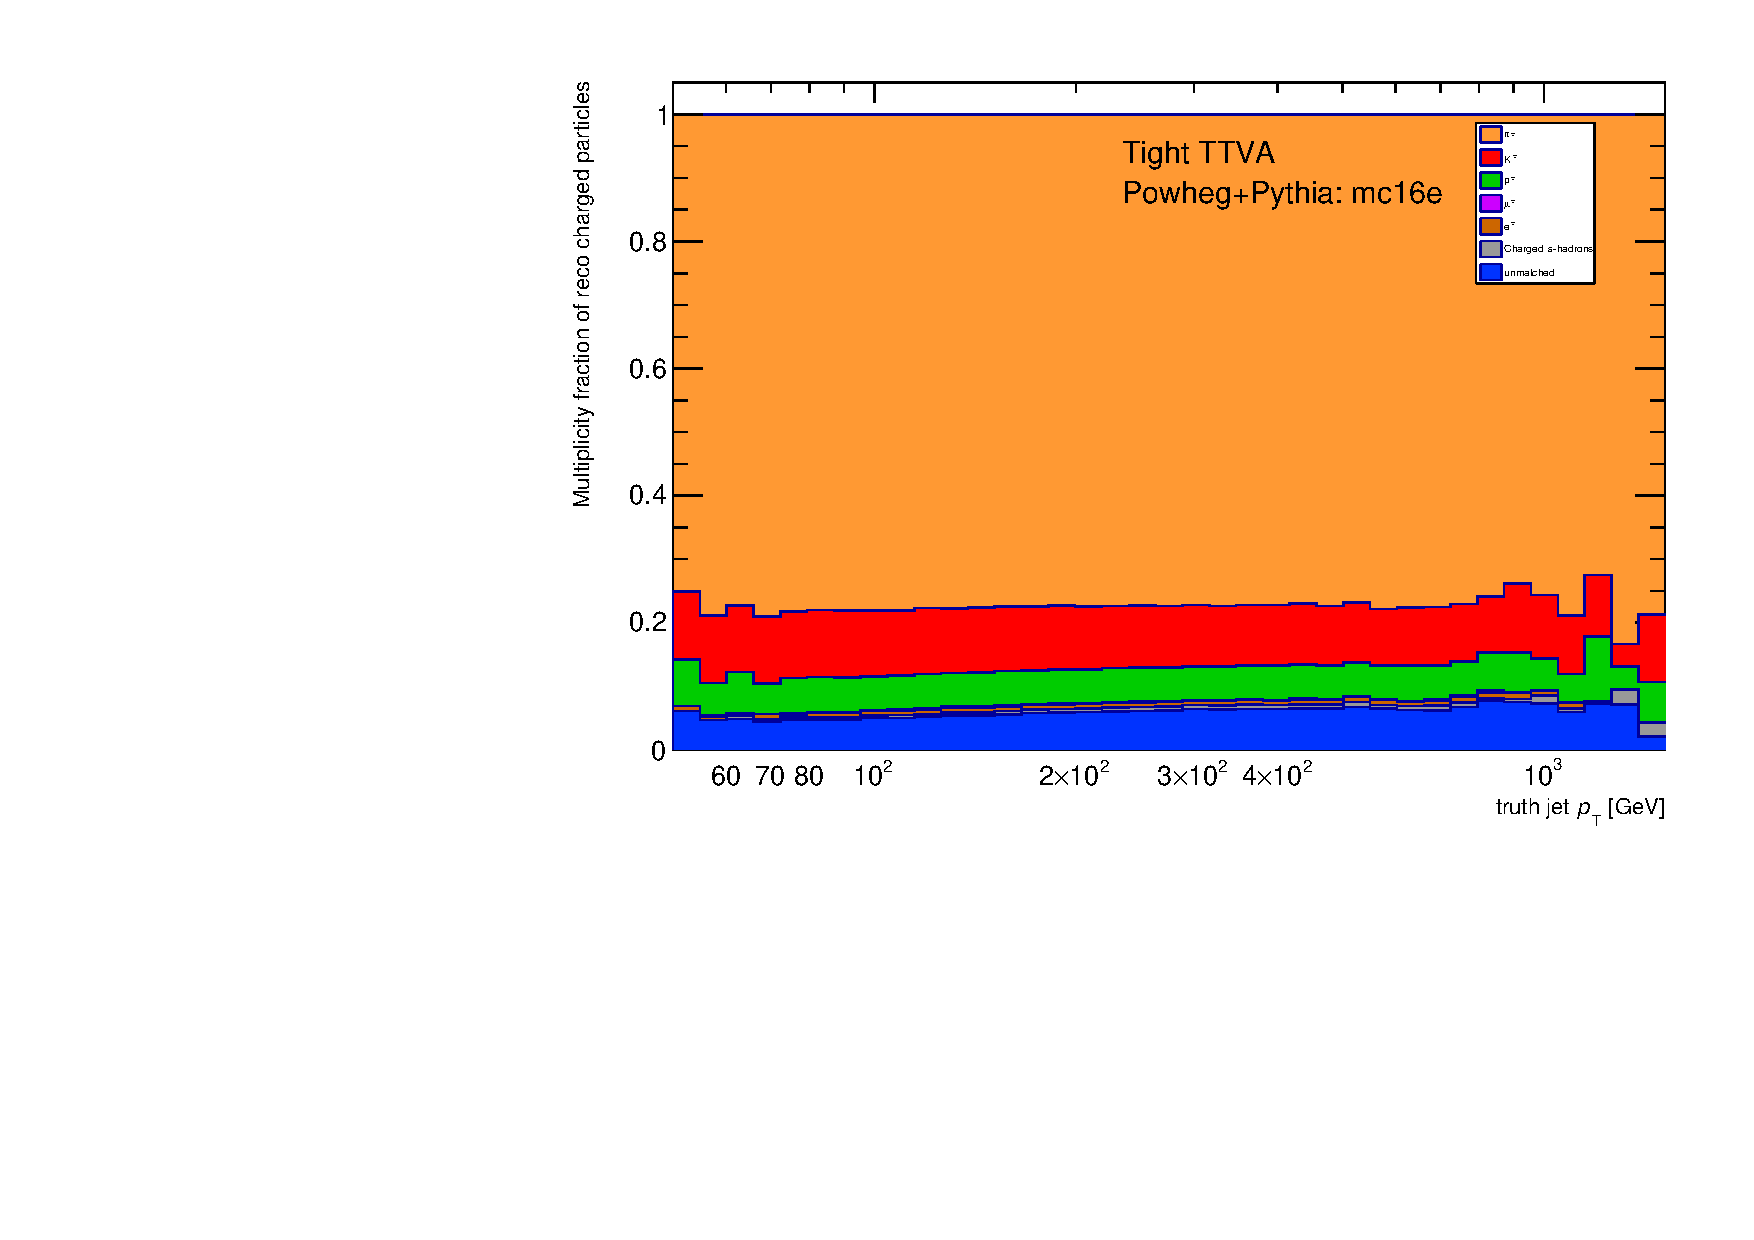
\includegraphics[width=0.48\textwidth,page=1]{figures/jetcompstudy_MultiplicityFraction.pdf}
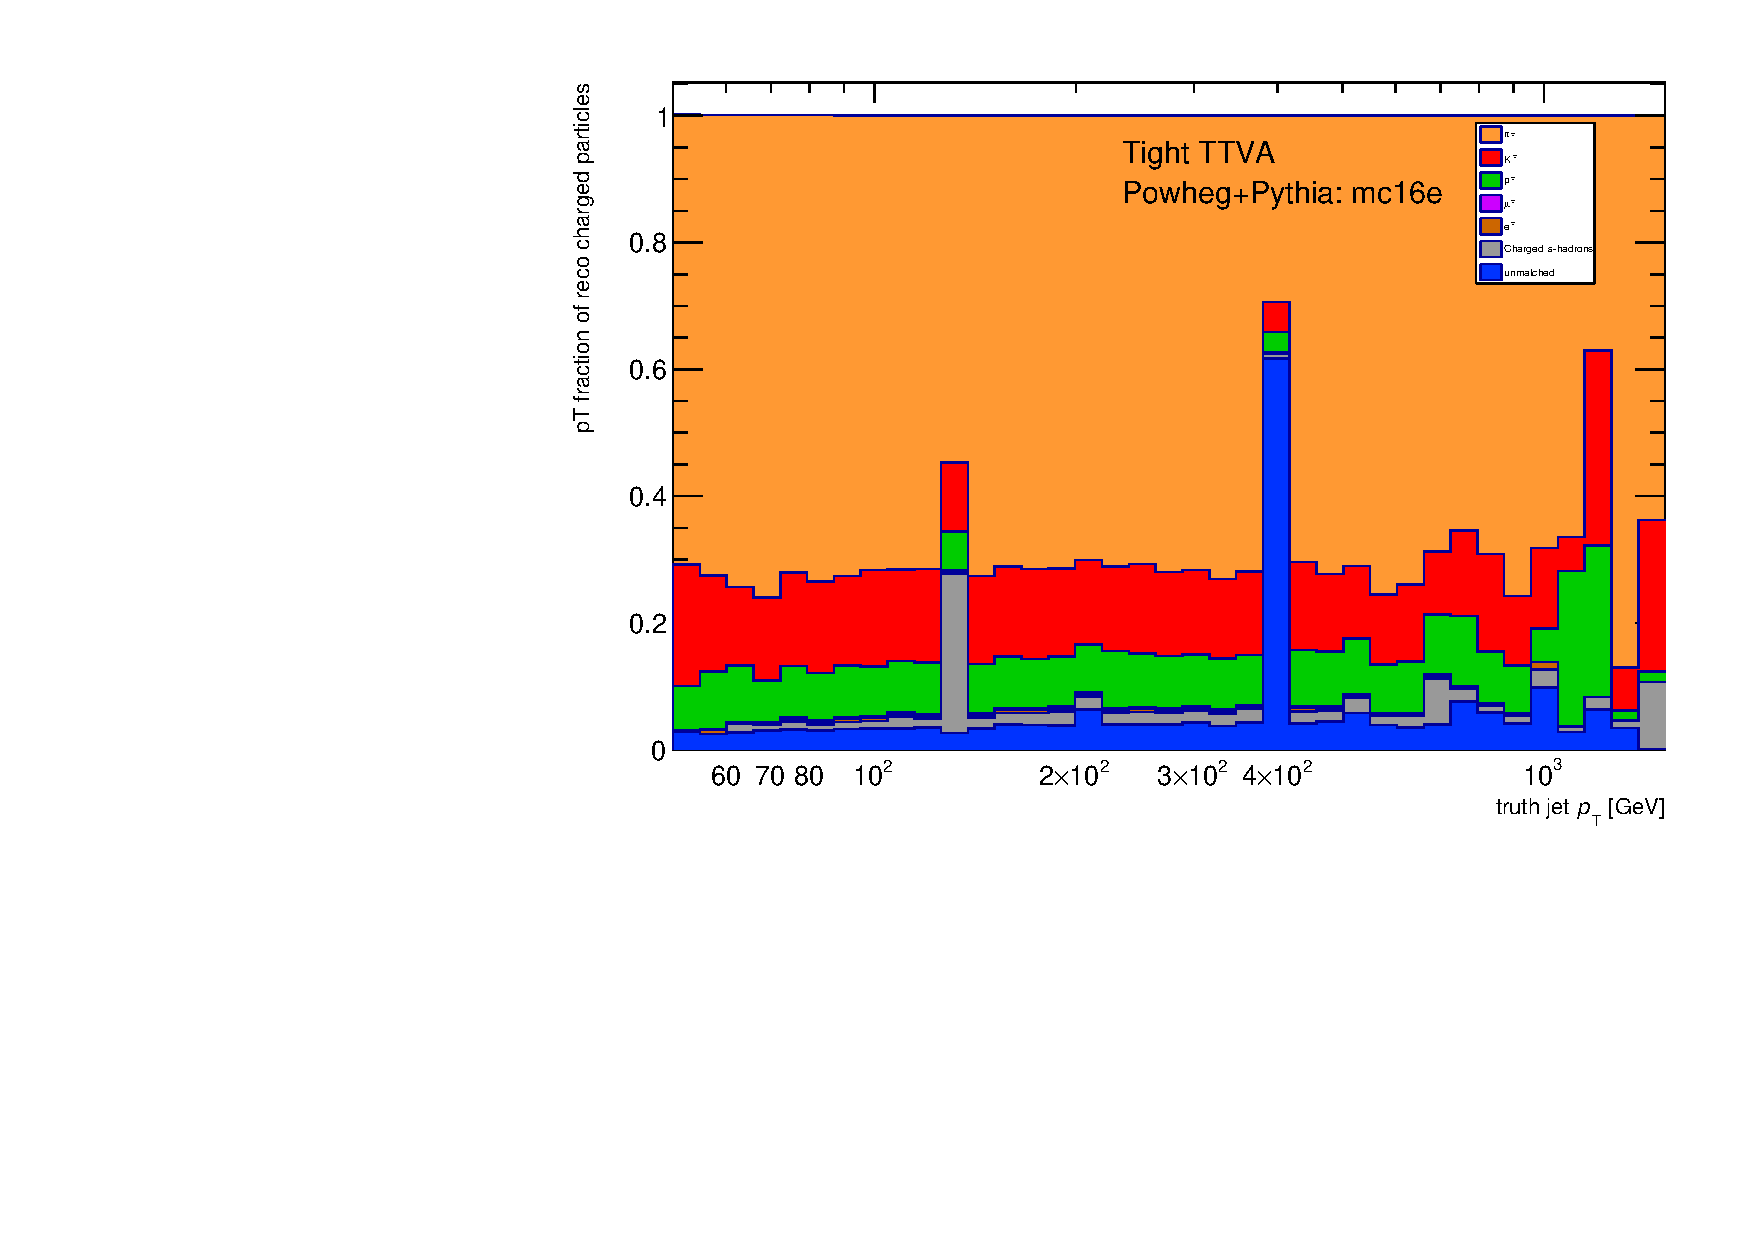
\includegraphics[width=0.48\textwidth,page=1]{figures/jet_comp_study_powheg_Tight_pTFraction_mc16e.pdf}%
\caption {The fraction of the reconstructed tracks multiplicity (left) and \pT (right) inside reconstructed leading jet as a function of jet pT for various categories. From charged particle compositions, mostly are pions $\approx71$\%, kaons are $\approx13$\% and rest $\approx16$\% comprise other charged particle.}
\label{fig:chargedparticles}
\end{figure}

Figure~\ref{fig:chargedparticles_truthjet} shows similar plots for all the charged particles compositions in the leading jet. 

\begin{figure}[b]
\centering
\includegraphics[scale=0.38, page=2]{figures/jetcompstudy_MultiplicityFraction.pdf}
\includegraphics[scale=0.38, page=2]{figures/jet_comp_study_powheg_Tight_pTFraction_mc16e.pdf}%
\caption {The fraction of the charged particle multiplicity (left) and \pT (right) inside particle level leading jet as a function of jet pT for various categories (see the text for details).}
\label{fig:chargedparticles_truthjet}
\end{figure}

Similarly, figures~\ref{fig:pions_kaons} to ~\ref{fig:electrons_sparticles} are showing the fraction of individual particles at truth level and reconstructed level. As shown in figure~\ref{fig:chargedparticles_truthjet}, pions make most of jet fraction, and for muons, electrons and strange particles this fraction is much lower. The muon and electron response is very low because these particles come from semi-leptonic decay of heavy hadrons, so we have a displaced vertex.

\begin{figure}[b]
\centering
\includegraphics[scale=0.3, page=10]{figures/jet_comp_study_powheg_Tight_pTFraction_mc16e.pdf}
\includegraphics[scale=0.3, page=11]{figures/jet_comp_study_powheg_Tight_pTFraction_mc16e.pdf}
\caption {The fraction of pions (left) and kaons (right) in the reconstructed tracks as a function of jet \pT, which shows  $\approx73$\% pions and $\approx14$\% kaons as reco level.}
\label{fig:pions_kaons}
\end{figure}

\begin{figure}[b]
\centering
\includegraphics[scale=0.3, page=12]{figures/jet_comp_study_powheg_Tight_pTFraction_mc16e.pdf}
\includegraphics[scale=0.3, page=13]{figures/jet_comp_study_powheg_Tight_pTFraction_mc16e.pdf}
\caption {The fraction of protons (left) and muons (right) in the reconstructed tracks as a function of jet \pT, which shows  $\approx7$\% proton at reco level and fraction of muons is very low.}
\label{fig:protons_muons}
\end{figure}

\begin{figure}[b]
\centering
\includegraphics[scale=0.3, page=14]{figures/jet_comp_study_powheg_Tight_pTFraction_mc16e.pdf}
\includegraphics[scale=0.3, page=15]{figures/jet_comp_study_powheg_Tight_pTFraction_mc16e.pdf}
\caption {The fraction of electrons (left) and strange particles (right) in the reconstructed tracks as a function of jet \pT.}
\label{fig:electrons_sparticles}
\end{figure}

\clearpage
